\documentclass[a4paper, 12pt]{article}

\usepackage{multirow}
\usepackage[table,xcdraw]{xcolor}
\usepackage{enumerate}
\usepackage{graphicx}
\usepackage[T5]{fontenc}
\usepackage[utf8]{inputenc}
\usepackage[margin = 2cm]{geometry}
\usepackage{amsfonts, amsmath, amssymb}
\usepackage[none]{hyphenat}
\usepackage{fancyhdr}
\usepackage{float}
\usepackage{hyperref}
\usepackage{caption}
\usepackage[nottoc, notlot, notlof]{tocbibind}

\captionsetup[table]{skip=5pt}
\pagestyle{fancy}
\fancyhead[L]{Trường Đại học Khoa học Tự nhiên - ĐHQG TP.HCM}
\fancyhead[R]{Nhóm Just $4^{th}$}

\begin{document}

\begin{titlepage}
	\begin{center}
		\vspace*{1cm}
		\Large\textbf{Báo cáo \#3\\Giao diện người dùng \& Kiểm thử}\\

		\vfill
		\line(1,0){450}\\[4mm]
		\LARGE\textbf{\MakeUppercase{Dự án quản lý tạp chiếu phim}}\\[3mm]
		\Large{Nhập môn Công nghệ phần mềm (CSC13002)}\\[3mm]
		\Large{Nhóm Just $4^{th}$}
		\line(1,0){430}\\
		\vfill

		\vfill
		TP Hồ Chí Minh, ngày 09/12/2020
	\end{center}
\end{titlepage}

\tableofcontents
\thispagestyle{empty}
\clearpage

\section{Thông tin nhóm}
\label{sec:info}
\begin{enumerate}
	\item \textbf{Đường link GitHub}: \url{https://github.com/baolongnguyenmac/CinemaManagementSystem}
	\item \textbf{Đường link Trello}: \url{https://trello.com/b/OmRBLunD/báo-cáo-giao-diện-kiểm-thử}
	\item \textbf{Danh sách thành viên}
	\begin{table}[H]
		\begin{center}
			\begin{tabular}{|c|c|l|c|c|}
				\hline
				STT & MSSV     & \multicolumn{1}{c|}{Họ tên} & Email                         & SĐT        \\ \hline
				1   & 18120201 & Nguyễn Bảo Long             & 18120201@student.hcmus.edu.vn & 0919070940 \\ \hline
				2   & 18120211 & Võ Thế Minh                 & 18120211@student.hcmus.edu.vn & 0981850699 \\ \hline
				3   & 18120227 & Phạm Văn Minh Phương        & 18120227@student.hcmus.edu.vn & 0343049359 \\ \hline
				4   & 18120210 & Phạm Tống Bình Minh         & 18120210@student.hcmus.edu.vn & 0971877781 \\ \hline
				5   & 18120264 & Nguyễn Duy Vũ               & 18120264@student.hcmus.edu.vn & 0911572108 \\ \hline
			\end{tabular}
			\caption{Bảng danh sách thành viên nhóm}
		\end{center}
	\end{table}
\end{enumerate}
\clearpage

\section{Lịch sử cập nhật}
\label{sec:history}
\begin{table}[h]
	\begin{center}
		\begin{tabular}{|c|c|c|l|l|}
			\hline
			STT &Ngày cập nhật &Phiên bản &\multicolumn{1}{c|}{Mô tả chi tiết} &\multicolumn{1}{c|}{Tác giả} \\ \hline
			1 &09/12/2020 &1.0 &\begin{tabular}[c]{@{}l@{}}- Lên kế hoach test\\- Lập bộ test\\- Đặc tả testcase\end{tabular} &\begin{tabular}[c]{@{}l@{}}Phạm Tống Bình Minh\\ Nguyễn Duy Vũ\end{tabular} \\ \hline
			2 &10/12/2020 &1.1 &\begin{tabular}[c]{@{}l@{}}- Vẽ sơ đồ điều hướng giữa các\\ màn hình\\- Đặc tả giao diện\\ - Cập nhật kế hoạch làm việc\\\end{tabular} &\begin{tabular}[c]{@{}l@{}}Phạm Văn Minh Phương\\ Nguyễn Bảo Long \\ Võ Thế Minh\end{tabular} \\ \hline
			3 &13/12/2020 &1.2 &\begin{tabular}[c]{@{}l@{}}- Quản trị dự án và kế hoạch \\làm việc\end{tabular} &\begin{tabular}[c]{@{}l@{}}Nguyễn Bảo Long\end{tabular} \\ \hline
			% 4 &30/10/2020 &1.3 &- Đặc tả giao diện người dùng &Phạm Văn Minh Phương \\ \hline
			% 5 &31/10/2020 &1.5 &- Phân tích đóng góp cá nhân &Phạm Văn Minh Phương \\ \hline
		\end{tabular}
		\caption{Bảng lịch sử cập nhật các phiên bản của báo cáo yêu cầu}
	\end{center}
\end{table}
\clearpage

\section{Phân tích đóng góp cá nhân}
\label{sec:analys}
\begin{table}[H]
	\begin{center}
		\begin{tabular}{|c|l|l|c|}
			\hline
			STT & \multicolumn{1}{c|}{Họ tên} & \multicolumn{1}{c|}{Công việc tham gia}                                                & Phần trăm đóng góp \\ \hline
			1 & Nguyễn Bảo Long      & \begin{tabular}[c]{@{}l@{}}- Tổng hợp báo cáo\\- Đặc tả giao diện \\- Thiết kế front-end hệ thống\\\end{tabular}              & 20\% \\ \hline
			2 & Phạm Văn Minh Phương & \begin{tabular}[c]{@{}l@{}}- Đặc tả giao diện\\ - Vẽ sơ đồ điều hướng giữa các màn hình\\- Thiết kế front-end hệ thống\\\end{tabular}                          & 20\% \\ \hline
			3 & Võ Thế Minh          & \begin{tabular}[c]{@{}l@{}}- Vẽ biểu đồ Gantt\\ - Thiết kế bản demo back-end hệ thống\end{tabular} & 20\%               \\ \hline
			4 & Phạm Tống Bình Minh  & \begin{tabular}[c]{@{}l@{}}- Thiết kế back-end hệ thống \\- Đặc tả testcase\\- Lập bộ test\\\end{tabular}               & 20\% \\ \hline
			5 & Nguyễn Duy Vũ        & \begin{tabular}[c]{@{}l@{}}- Lên kế hoạch test\\ - Đặc tả testcase\end{tabular} & 20\% \\ \hline
		\end{tabular}
		\caption{Bảng phân tích đóng góp cá nhân}
	\end{center}
\end{table}
\clearpage

\section{Thiết kế giao diện người dùng}

\subsection{Sơ đồ và điều hướng giữa các màn hình}

\subsection{Đặc tả màn hình giao diện}

\clearpage

\section{Kiểm thử phần mềm}

\subsection{Kế hoạch kiểm thử}

\subsection{Test case}

\subsubsection{Danh sách test case}

\subsubsection{Đặc tả test case}

\clearpage

\section{Quản trị dự án và kế hoạch làm việc}

\subsection{Báo cáo tiến độ}

\begin{itemize}
	\item Các công việc đã hoàn thành
	\begin{itemize}
		\item Xác thực đặt vé, huỷ vé, quản lý thông tin phim phía back-end
		\item Giao diện chức năng đặt vé, huỷ vé
	\end{itemize}
	\item Công việc chưa hoàn thành: Giao diện chức năng quản lý thông tin phim 

	\item Tính tới thời điểm hiện tại, mọi công việc đều đang đi đúng theo tiến độ
	\item Giải pháp làm việc việc đúng tiến độ: Tận dụng thời gian để học công nghệ liên quan đến các công việc cần làm và thực hành nháp để quen với công nghệ mới sau đó bắt tay vào thực hiện công việc
\end{itemize}

\clearpage 

\subsection{Kế hoạch thực hiện}

\begin{itemize}
	\item ID của các tác vụ và các milestone được giải thích chi tiết trong báo cáo 1
	\item Biểu đồ Gantt 
	\begin{figure}[H]
		\begin{center}
			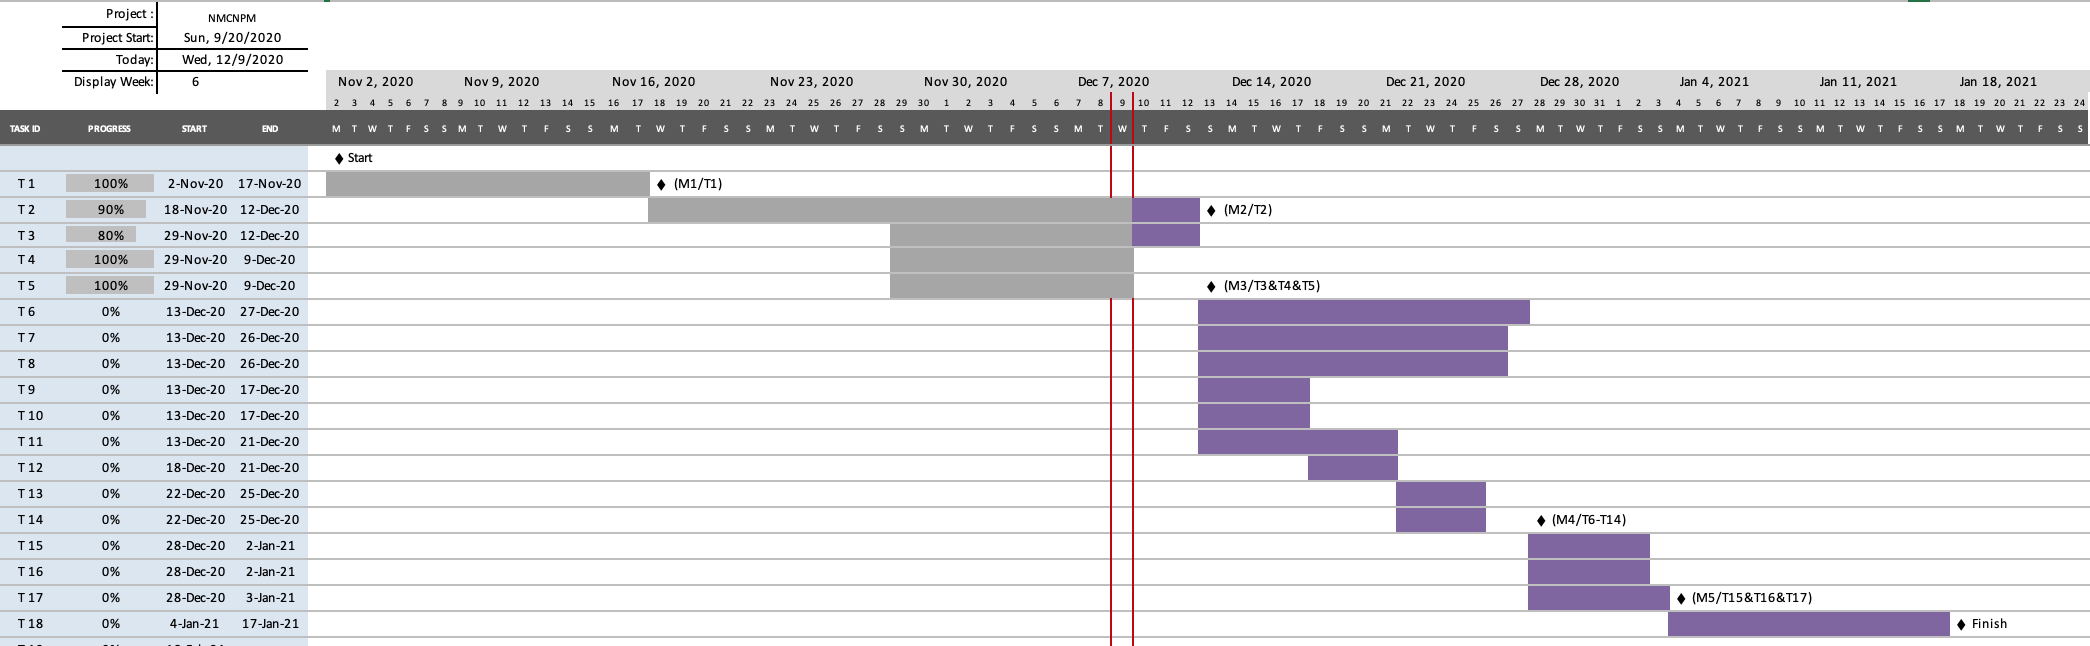
\includegraphics[scale=0.59, angle=90]{./image/gantt.png}
			\caption{Biểu đồ Gantt}
		\end{center}
	\end{figure}
\end{itemize}

\subsection{Phân rã trách nhiệm}

\begin{itemize}
	\item Từ ngày 18/11/2020 đến ngày 12/12/2020, các thành viên trong nhóm chịu trách nhiệm cho các công việc sau
	\begin{table}[H]
		\begin{center}
			\begin{tabular}{|c|l|l|}
			\hline
			STT & \multicolumn{1}{c|}{Họ tên} & \multicolumn{1}{c|}{Công việc}                         \\ \hline
			1 & \multirow{3}{*}{\begin{tabular}[c]{@{}l@{}}- Nguyễn Bảo Long\\ - Phạm Văn Minh Phương\end{tabular}} & Thiết kế giao diện chức năng Huỷ vé    \\ \cline{1-1} \cline{3-3} 
			2   &                             & Thiết kế giao diện chức năng Đặt vé                    \\ \cline{1-1} \cline{3-3} 
			3   &                             & Thiết kế giao diện chức năng Quản lý thông tin phim    \\ \hline
			4 & \multirow{3}{*}{\begin{tabular}[c]{@{}l@{}}- Võ Thế Minh\\ - Phạm Tống Bình Minh\end{tabular}}      & Thiết kế back-end cho chức năng Đặt vé \\ \cline{1-1} \cline{3-3} 
			5   &                             & Thiết kế back-end cho chức năng Huỷ vé                 \\ \cline{1-1} \cline{3-3} 
			6   &                             & Thiết kế back-end cho chức năng Quản lý thông tin phim \\ \hline
			4   & - Nguyễn Duy Vũ             & Triển khai kiểm thử                                    \\ \hline
			\end{tabular}
			\caption{Bảng phân rã trách nhiệm đối với từng công việc cụ thể}
		\end{center}
	\end{table}

	\item Thành viên điều phối việc tích hợp: Phạm Tống Bình Minh 
	\item Thành viên điều phối việc kiểm thử tích hợp: Nguyễn Duy Vũ
\end{itemize}

\clearpage

\section{Tham khảo}

\end{document}